\subsection{Anmerkungen zur Auswertung}
Im Folgenden wird der Einfluss jedes Parameters exemplarisch für eine Auswahl an Systemen gezeigt, da der zu beobachtende Trend für alle drei Systeme ähnlich ausfällt.

\begin{figure}[hb] %sim
	\centering
	\begin{subfigure}{0.5\textwidth}
	  \centering
	  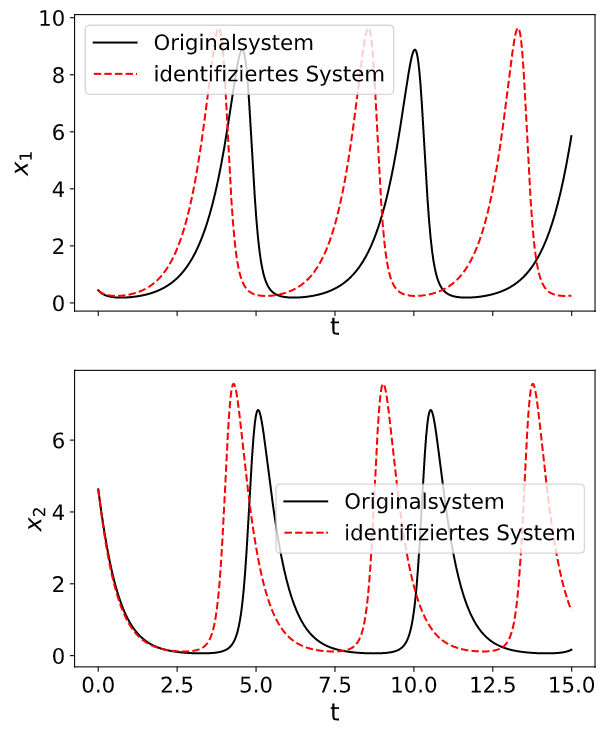
\includegraphics[width=75mm]{images/sim_volterra_e_0_1_sim.png}
	  \caption{Simulationsverlauf}
	  \label{fig:sim_volterra_e_0.1_sim}
	\end{subfigure}%
	\begin{subfigure}{.5\textwidth}
	  \centering
	  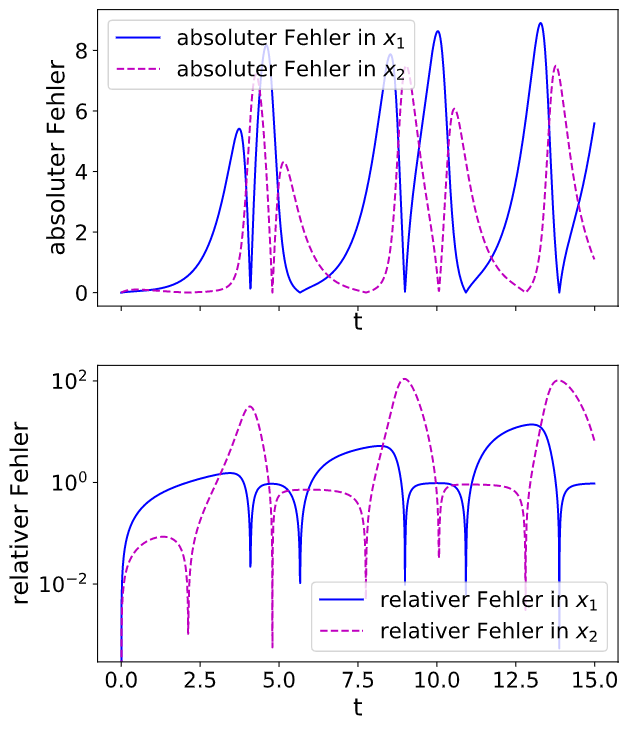
\includegraphics[width=75mm]{images/sim_volterra_e_0_1_err.png}
	  \caption{Fehlerverlauf}
	  \label{fig:sim_volterra_e_0.1_err}
	\end{subfigure}
	\caption{Simulation des Lotka-Volterra-Systems, relativer Fehler der identifizierten Koeffizienten $\varepsilon_\text{r} = 10 \%. $ }
	\label{fig:sim_volterra_e_0.1}
\end{figure}
\begin{figure}[h] %sim
	\centering
	\begin{subfigure}{.5\textwidth}
	  \centering
	  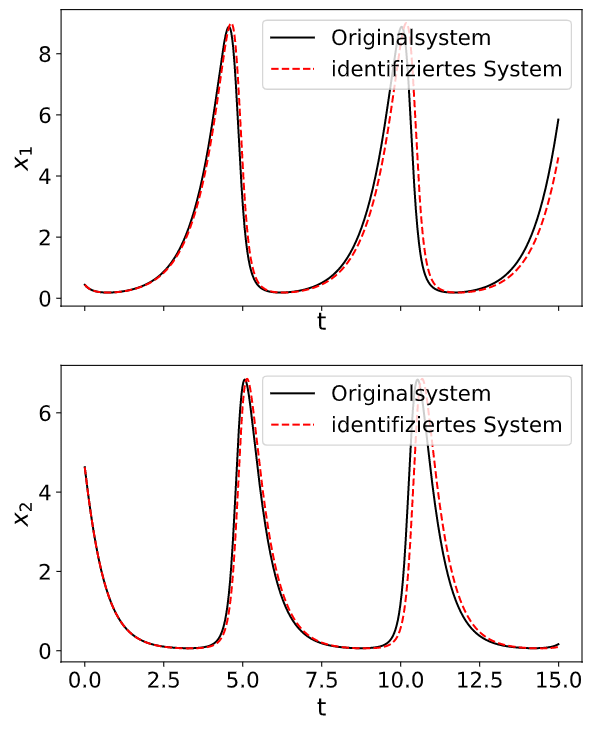
\includegraphics[width=75mm]{images/sim_volterra_e_0_01_sim.png}
	  \caption{Simulationsverlauf}
	  \label{fig:sim_volterra_e_0.01_sim}
	\end{subfigure}%
	\begin{subfigure}{.5\textwidth}
	  \centering
	  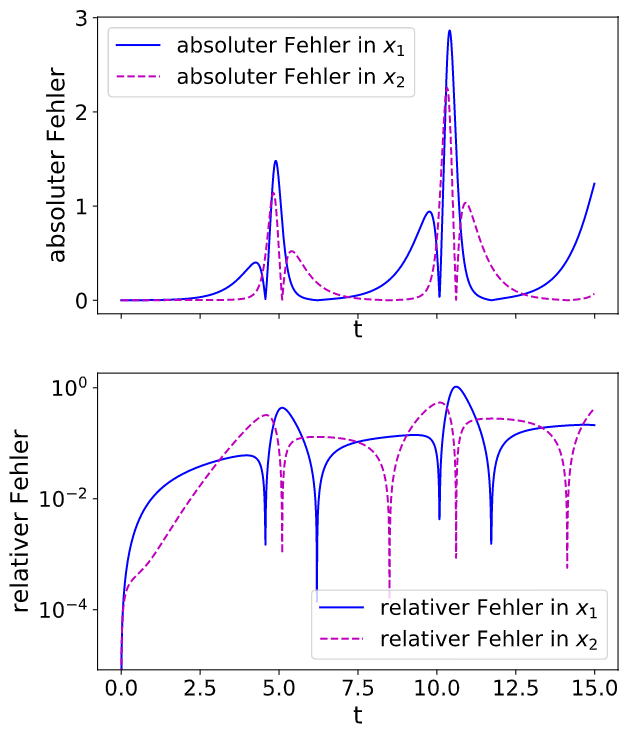
\includegraphics[width=75mm]{images/sim_volterra_e_0_01_err.png}
	  \caption{Fehlerverlauf}
	  \label{fig:sim_volterra_e_0.01_err}
	\end{subfigure}
	\caption{Simulation des Lotka-Volterra-Systems, relativer Fehler der identifizierten Koeffizienten $\varepsilon_\text{r} = 1 \%. $ }
	\label{fig:sim_volterra_e_0.01}
\end{figure}
\begin{figure}[h] %sim
	\centering
	\begin{subfigure}{.5\textwidth}
	  \centering
	  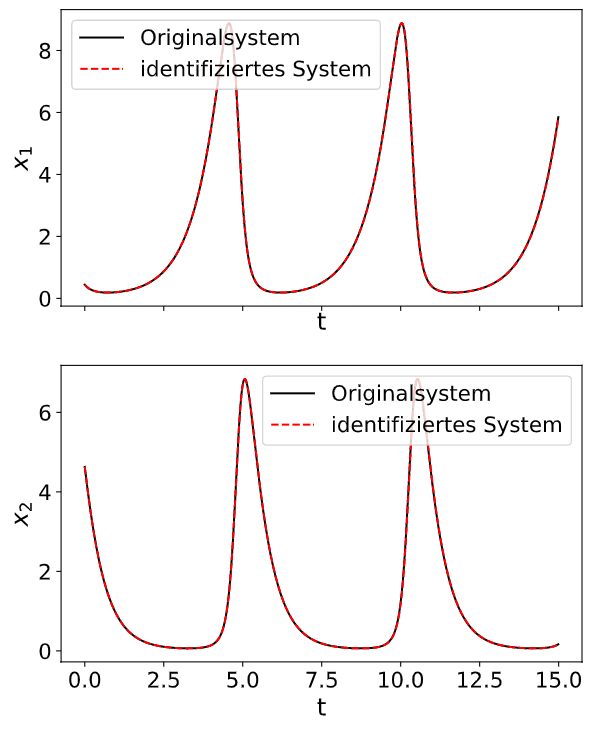
\includegraphics[width=75mm]{images/sim_volterra_e_0_001_sim.png}
	  \caption{Simulationsverlauf}
	  \label{fig:sim_volterra_e_0.001_sim}
	\end{subfigure}%
	\begin{subfigure}{.5\textwidth}
	  \centering
	  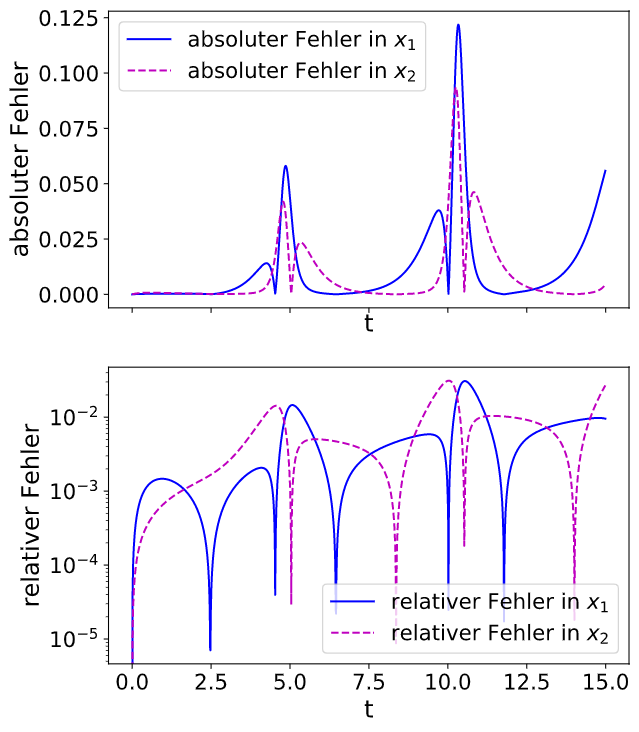
\includegraphics[width=75mm]{images/sim_volterra_e_0_001_err.png}
	  \caption{Fehlerverlauf}
	  \label{fig:sim_volterra_e_0.001_err}
	\end{subfigure}
	\caption{Simulation des Lotka-Volterra-Systems, relativer Fehler der identifizierten Koeffizienten $\varepsilon_\text{r} = 0.1 \%.  $ }
	\label{fig:sim_volterra_e_0.001}
\end{figure}

Um die nachfolgend gezeigten Fehler in den identifizierten Koeffizienten in Relation setzen zu können, ist es sinnvoll, einen Blick auf Simulationen der identifizierten Systeme zu werfen. Abb. \ref{fig:sim_volterra_e_0.1},  \ref{fig:sim_volterra_e_0.01} und \ref{fig:sim_volterra_e_0.001} zeigen die Simulation des Lotka-Volterra-Systems mit unterschiedlich gut identifizierten Koeffizienten. Je kleiner der relative Fehler $\varepsilon_r$ der Koeffizienten ist, desto länger kann das identifizierte System als gute Näherung für das Originalsystem genutzt werden. Wie lange dies der Fall sein soll ist im Einzelfall von der gegebenen Anwendung abhängig und gibt damit auch eine Vorgabe für den maximal erlaubten Fehler der identifizierten Koeffizienten. Im Folgenden wird ein Identifikationsfehler $\varepsilon_\text{r}$ als klein und damit die Identifikation als erfolgreich befunden, wenn $\varepsilon_\text{r} < 1\%$. 

Der relative Fehler der Nominalableitungen zeigt den geringstmöglichen Fehler, den die Methode theoretisch erzielen könnte, wenn die Messungen der Zustandsableitungen exakt wären. Ist dieser Fehler null, so ist unter den gegebenen Parametern eine Systemidentifikation prinzipiell möglich. Im Praxisfall ist der Erfolg der Identifikation jedoch weiterhin von einem geeigneten Zusammenspiel zwischen Algorithmus-Parametern und den Messfehlern in den Datenreihen abhängig. Ist der Fehler bereits im Nominalfall nicht klein genug, so ist eine Identifikation bei Verwendung der Zentraldifferenz nicht möglich. Das deutet darauf hin, dass die Algorithmus-Parameter ungünstig gewählt sind.




Es wird der Einfluss der nachfolgenden Parameter auf das Identifikationsergebnis untersucht. Für die Untersuchung werden Standardwerte festgelegt, die konstant bleiben, während der zu untersuchende Parameter verändert wird. Diese werden in eckigen Klammer angegeben.
\begin{itemize}
\item die Simulationszeit $t$ des DGL-Lösers, [3s],
\item die Schrittweite $dt$ des DGL-Lösers, [0.01s], 
%\item die Anzahl der gleichzeitig analysierten Datenreihen, [eine Datenreihe],
\item die Gestaltung der Bibliothek von Ansatzfunktionen, [Polynome maximal zweiter Ordnung],
%\item das verwendete Optimierungsverfahren zur Lösung des Approximationsproblems, [rekursive MKQ]
\item die Stärke des Rauschens in den Daten, [kein Rauschen].
\end{itemize}
Die Standardparameter sind so gewählt, dass der resultierende Fehler für alle Systeme bereits klein ist. Die Veränderung eines Parameters kann dann den Bereich zeigen, in dem dieser noch sinnvoll verändert werden kann.

\subsection{Einfluss der Simulationszeit}
Wie aus Abb. \ref{fig:errors_tspan} hervorgeht, sinkt der relative Fehler der identifizierten Parameter bei Verwendung der Zentraldifferenz mit steigender Simulationszeit. Dabei ist auffällig, dass für zu geringe Simulationszeiten keine Systemidentifikation möglich ist, während sich der Fehler ab einer gewissen Mindestsimulationszeit kaum noch verändert. Diese Mindestzeit ist notwendig, damit charakteristische Zustandsverläufe sichtbar werden, ähnlich wie die Sinusfunktion mit der Winkelhalbierenden verwechselt werden kann, wenn das Betrachtungsfenter ungünstig gewählt wird. Allerdings sinkt der Fehler für große Simulationszeiten nicht mehr signifikant. Damit existiert für jedes System eine optimale Simulationsdauer.
\begin{figure} %errors tspan
	\centering
%	\begin{subfigure}{.5\textwidth}
%	  \centering
%	  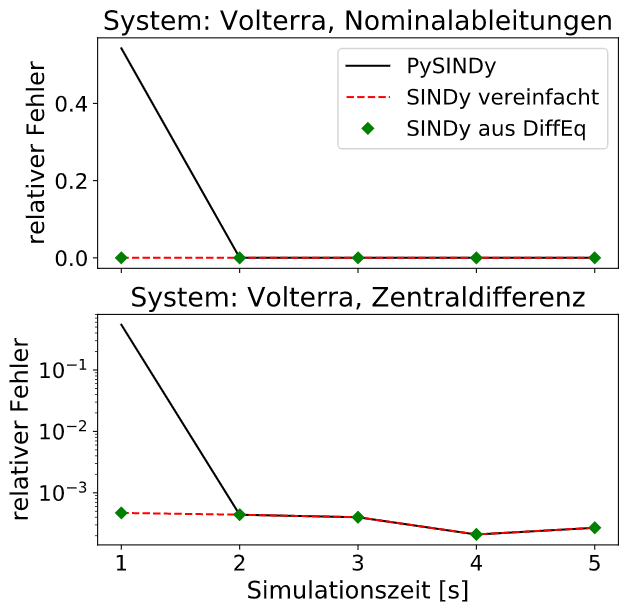
\includegraphics[width=75mm]{images/errors_volterra_tspan_variation.png}
%	  \caption{Lotka-Volterra-System}
%	  \label{fig:errors_volterra_tspan}
%	\end{subfigure}%
%	\begin{subfigure}{.5\textwidth}
%	  \centering
	  \includegraphics[width=75mm]{images/errors_roessler_tspan_variation.png}
%	  \caption{Rössler-System}
%	  \label{fig:errors_roessler_tspan}
%	\end{subfigure}
	\caption{relativer Fehler der identifizierten Parameter in Abhängigkeit der Simulationszeit.}
	\label{fig:errors_tspan}
\end{figure}

\subsection{Einfluss der Simulationsschrittweite}
Um Anforderungen an die Messung der Zustandskomponenten zu minimieren, ist es sinnvoll zu fordern, dass die Zeit zwischen zwei Messungen (hier durch die Simulationsschrittweite repräsentiert) so groß wie möglich gewählt wird. In Abb. \ref{fig:errors_dt} zeigt sich, dass der Fehler mit zunehmender Schrittweite steigt. Jedes System besitzt eine spezifische Schrittweite, ab welcher keine Identifikation mehr möglich ist. Anders als bei der Simulationszeit sinkt der Fehler hier für kleine Schrittweiten immer weiter, bis hin zum Extremfall, dass die Schrittweite infinitesimal klein ist und der Fehler null wird (siehe Nominalfall). Damit muss man bei der Auswahl der Schrittweite zwischen Genauigkeit und Messaufwand abwägen.
\begin{figure} %errors dt
	\centering
	\begin{subfigure}{.5\textwidth}
	  \centering
	  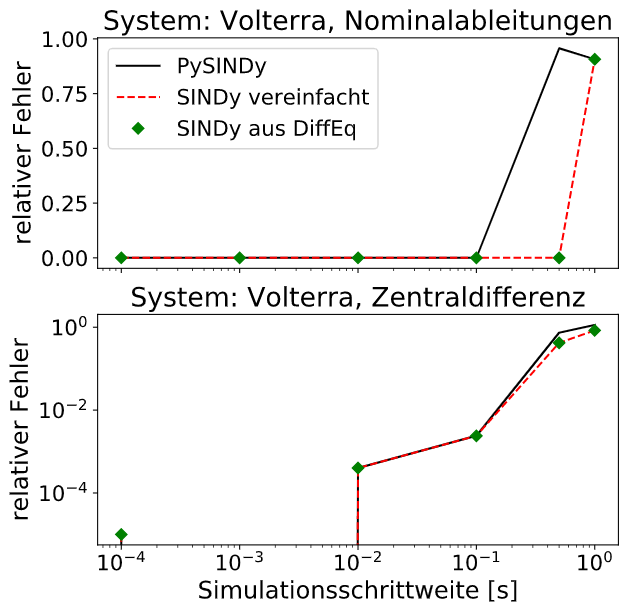
\includegraphics[width=75mm]{images/errors_volterra_dt_variation.png}
	  \caption{Lotka-Volterra-System}
	  \label{fig:errors_volterra_dt}
	\end{subfigure}%
	\begin{subfigure}{.5\textwidth}
	  \centering
	  \includegraphics[width=75mm]{images/errors_lorenz_dt_variation.png}
	  \caption{Lorenz-System}
	  \label{fig:errors_lorenz_dt}
	\end{subfigure}
	\caption{relativer Fehler der identifizierten Parameter in Abhängigkeit der Simulationsschrittweite.}
	\label{fig:errors_dt}
\end{figure}

\subsection{Einfluss der Gestaltung der Bibliothek}
Wie bereits angedeutet ist die Auslegung der Bibliothek entscheidend für eine erfolgreiche Identifikation. Je weniger Informationen dem Algorithmus im Vorhinein zur Verfügung gestellt werden müssen, desto mächtiger ist er. Daher ist es wünschenswert, die Bibliothek so groß wie möglich ansetzen zu können, um auch Funktionsklassen zu beinhalten, deren Vorkommen nicht gesichert ist. Für die drei zu untersuchenden Systeme wurde eine polynomiale Bibliothek angesetzt, die schrittweise durch Monome höherer Ordnung ergänzt wurde. Abb. \ref{fig:errors_order} zeigt, dass die Bibliothek mit deutlich mehr Funktionen besetzt werden kann als nötig und eine Identifikation trotzdem noch möglich ist. Allerdings gibt es auch hier einen Punkt, ab dem die Identifikation scheitert. Mit zunehmender Anzahl an Funktionen wird es wahrscheinlicher, dass eine Linearkombination dieser Funktionen existiert, die eine in der DGL vorkommende Funktion hinreichend genau beschreibt und ein Teil des Ergebnisses wird. Die so entstandene DGL kann das System in der Regel ausreichend gut numerisch modellieren, ist aber auf Grund der falsch identifizierten Ansatzfunktionen nur als Black-Box-Modell zu gebrauchen und für die Identifikation von analytischen Zusammenhängen unbrauchbar.

\begin{figure}[h!] %errors order
	\centering
	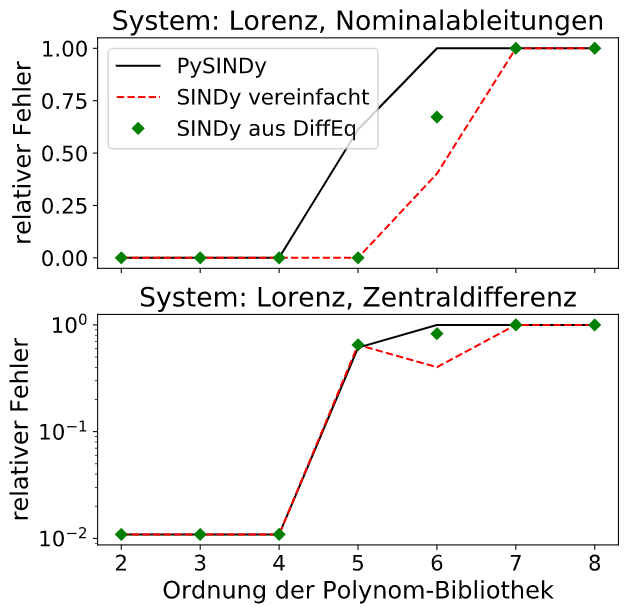
\includegraphics[width=75mm]{images/errors_Lorenz_order_variation.png}
	\caption{relativer Fehler der Identifizierten Parameter in Abhängigkeit der Ordnung der Polynom-Bibliothek.}
	\label{fig:errors_order}
\end{figure}

\subsection{Einfluss von verrauschten Daten}
Für die folgende Untersuchung (Abb. \ref{fig:errors_noise}) wurden die Verläufe der Zustandskomponenten mit additivem weißen Rauschen überlagert. Die Stärke des Rauschsignals wurde über die Standardabweichung der verwendeten Normalverteilung eingestellt. Je stärker das Rauschen, desto ungenauer werden die identifizierten Koeffizienten. Wie stark verrauscht die Daten sein können, sodass dennoch eine Identifikation möglich ist, hängt vom System ab.
\begin{figure}[h!] %errors noise
	\centering
	\begin{subfigure}{.5\textwidth}
	  \centering
	  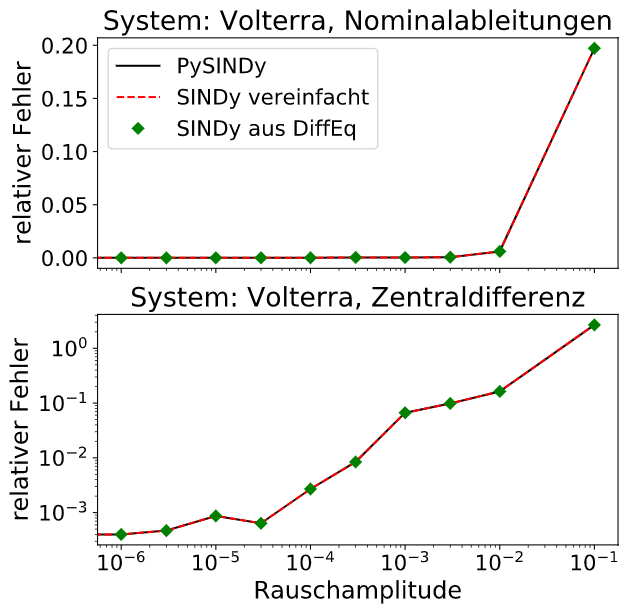
\includegraphics[width=75mm]{images/errors_volterra_noise_variation.png}
	  \caption{Lotka-Volterra-System}
	  \label{fig:errors_volterra_noise}
	\end{subfigure}%
	\begin{subfigure}{.5\textwidth}
	  \centering
	  \includegraphics[width=75mm]{images/errors_lorenz_noise_variation.png}
	  \caption{Lorenz-System}
	  \label{fig:errors_lorenz_noise}
	\end{subfigure}
	\caption{relativer Fehler der identifizierten Parameter in Abhängigkeit der Rauschstärke.}
	\label{fig:errors_noise}
\end{figure}

\subsection{Rechenzeit}
Abb. \ref{fig:time} zeigt exemplarisch das qualitative Verhältnis der Rechenzeiten der Implementationen. Beide \textit{Python}-Implementationen sind deutlich schneller als die \textit{Julia}-Version. Dennoch ist die Rechenzeit in allen Fällen recht klein. Der vereinfachte Algorithmus schneidet am besten ab, was damit zu erklären ist, dass viele periphere Funktionen, wie die Validierung der Eingabedaten, nicht implementiert sind.

\begin{figure}[h!] %times
	\centering
	\begin{subfigure}{.5\textwidth}
	  \centering
	  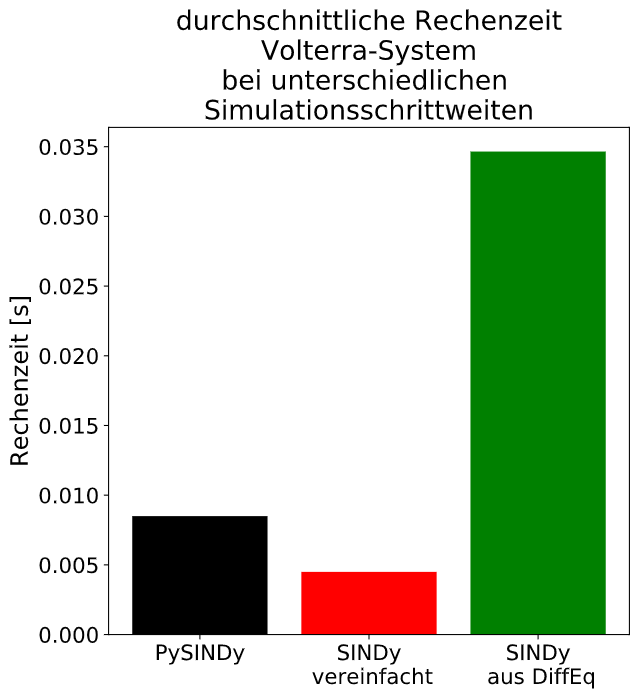
\includegraphics[width=75mm]{images/time_volterra_dt.png}
	  %\caption{Lotka-Volterra-System}
	%  \label{fig:time_volterra_dt}
	\end{subfigure}%
	\begin{subfigure}{.5\textwidth}
	  \centering
	  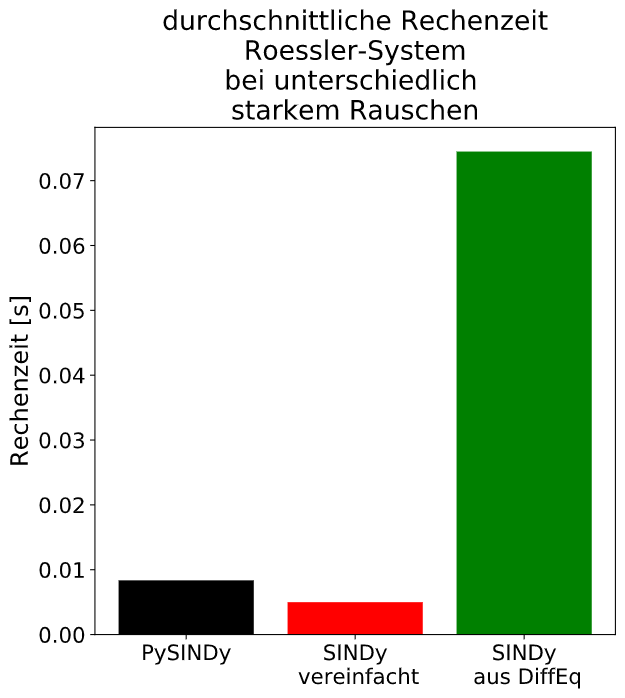
\includegraphics[width=75mm]{images/time_roessler_noise.png}
	  %\caption{Roessler-System}
	 % \label{fig:time_roessler_noise}
	\end{subfigure}
	\caption{durchschnittliche Rechenzeit der unterschiedlichen Algorithmen.}
	\label{fig:time}
\end{figure}


\subsection{Zusammenfassung der Ergebnisse}
Anders als zu Beginn der Arbeit vermutet, lassen sich keine Unterschiede in der Genauigkeit der SINDy-Implementationen feststellen. Allerdings ist die richtige Wahl der Parameter von großer Bedeutung für die Qualität der Identifikation. Die identifizierten Parameter werden genauer, wenn mehr Messdaten zur Verfügung stehen, also die Anzahl der Messungen steigt und der zeitliche Abstand zwischen ihnen verringert wird. Der Algorithmus kann mit verrauschten Messdaten arbeiten, genauere Messungen liefern bessere Ergebnisse. Die Bibliothek aus Ansatzfunktionen muss groß genug sein, um alle in den Systemgleichungen vorkommenden Ansatzfunktionen zu beinhalten und gleichzeitig klein genug, damit die Richtigen ausgewählt werden. Leider sind die optimalen Parameter von System zu System unterschiedlich, sodass hier keine allgemeingültigen Aussagen zur Größe von Parametern getroffen werden können.

